\newpage
\subsection{Caso d'uso UC10: Modalità allenamento}
\label{UC10}
	\begin{figure}[ht]
	\centering
	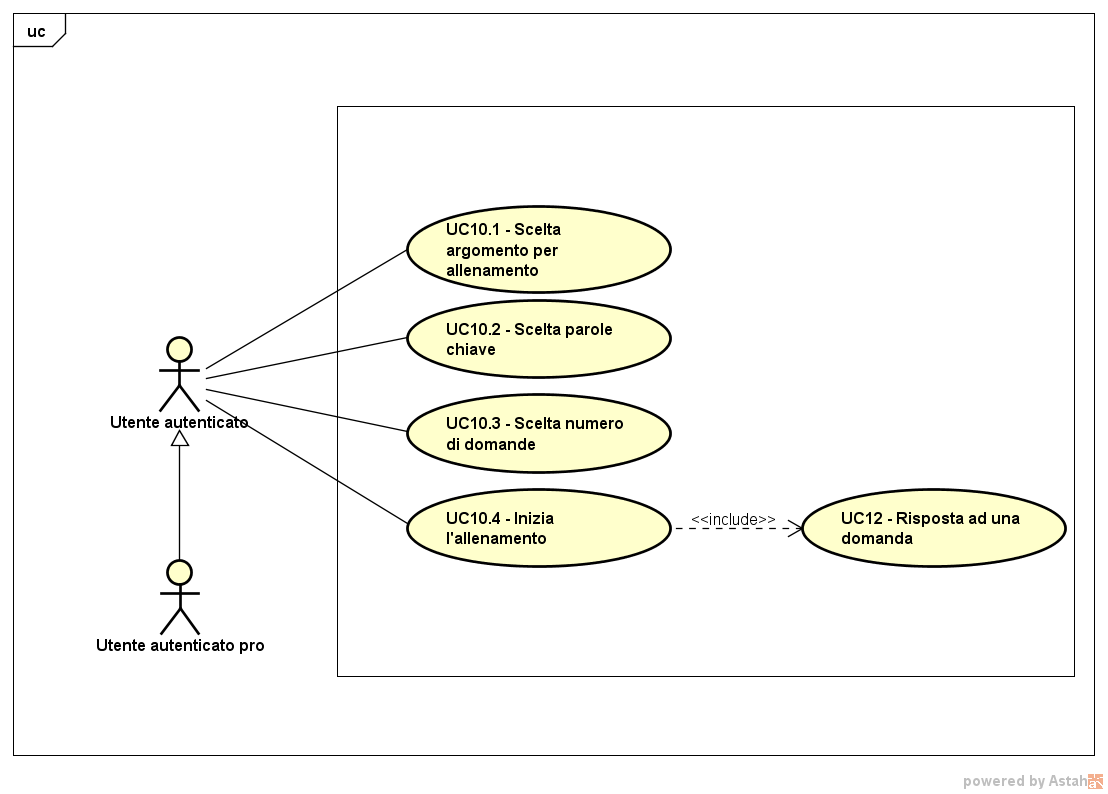
\includegraphics[scale=0.5]{UML/UC10.png}
	\caption{UC10: Modalità allenamento}
	\end{figure}
\FloatBarrier
\begin{itemize}
\item\textbf{Attori}: utente non autenticato, utente autenticato, utente autenticato pro;
\item\textbf{Descrizione}: l'attore può svolgere un allenamento che consiste nel rispondere a domande che gli vengono proposte in modo dinamico. La difficoltà di ogni domanda viene calcolata in modo che essa sia sempre in linea con la competenza dell'utente sull'argomento scelto;
\item\textbf{Precondizione}: l'attore ha selezionato l'opzione di allenamento;
\item\textbf{Postcondizione}: l'attore ha finito di svolgere l'allenamento e può quindi visualizzare la valutazione finale che ha ottenuto e il riepilogo delle risposte date nonché il proprio livello sugli argomenti;
\item\textbf{Scenario principale}:
	\begin{enumerate}
		\item L'attore può scegliere l'argomento per iniziare l'allenamento (UC10.1);
		\item L'attore può scegliere delle parole chiave (UC10.2);
		\item L'attore può scegliere il numero di domande che compongono l'allenamento (UC10.3);
		\item L'attore può iniziare l'allenamento (UC10.4).
	\end{enumerate}
\item \textbf{Inclusioni}: l'attore risponde ad una domanda (UC12).
\end{itemize}

\subsubsection{Caso d'uso UC10.1: Scelta argomento per l'allenamento}
	\begin{itemize}
		\item \textbf{Attori}: utente non autenticato, utente autenticato, utente autenticato pro;
		\item \textbf{Descrizione}: l'attore può scegliere l'argomento delle domande che compariranno nell'allenamento;
		\item \textbf{Precondizione}: l'attore ha selezionato la modalità allenamento;
		\item \textbf{Postcondizione}: l'attore ha scelto un argomento per l'allenamento;
		\item \textbf{Scenario Principale}: l'attore sceglie l'argomento sul quale vuole allenarsi.
	\end{itemize}
	
\subsubsection{Caso d'uso UC10.2: Scelta parole chiave}
	\begin{itemize}
		\item \textbf{Attori}: utente non autenticato, utente autenticato, utente autenticato pro;
		\item \textbf{Descrizione}: l'attore può scegliere le parole chiave, ovvero degli argomenti più specifici, delle domande che compariranno nell'allenamento;
		\item \textbf{Precondizione}: l'attore ha selezionato la modalità allenamento;
		\item \textbf{Postcondizione}: l'attore ha scelto delle parole chiave;
		\item \textbf{Scenario principale}: l'attore sceglie delle parole chiave per filtrare in modo più dettagliato possibile l'argomento delle domande proposte per l'allenamento.
	\end{itemize}
	
\subsubsection{Caso d'uso UC10.3: Scelta numero di domande}
	\begin{itemize}
		\item \textbf{Attori}: utente non autenticato, utente autenticato, utente autenticato pro;
		\item \textbf{Descrizione}: l'attore può scegliere il numero di domande che comporranno l'allenamento, senza restrizione sul numero;
		\item \textbf{Precondizione}: l'attore ha selezionato la modalità allenamento;
		\item \textbf{Postcondizione}: l'attore ha scelto il numero di domande che comporranno l'allenamento;
		\item \textbf{Scenario principale}: l'attore sceglie il numero di domande che comporranno l'allenamento;
		\item \textbf{Scenari alternativi}: l'attore non sceglie un numero di domande che saranno quindi infinite.
	\end{itemize}
	
\subsubsection{Caso d'uso UC10.4: Inizia allenamento}
\label{UC10.4}
\begin{figure}
	\centering
	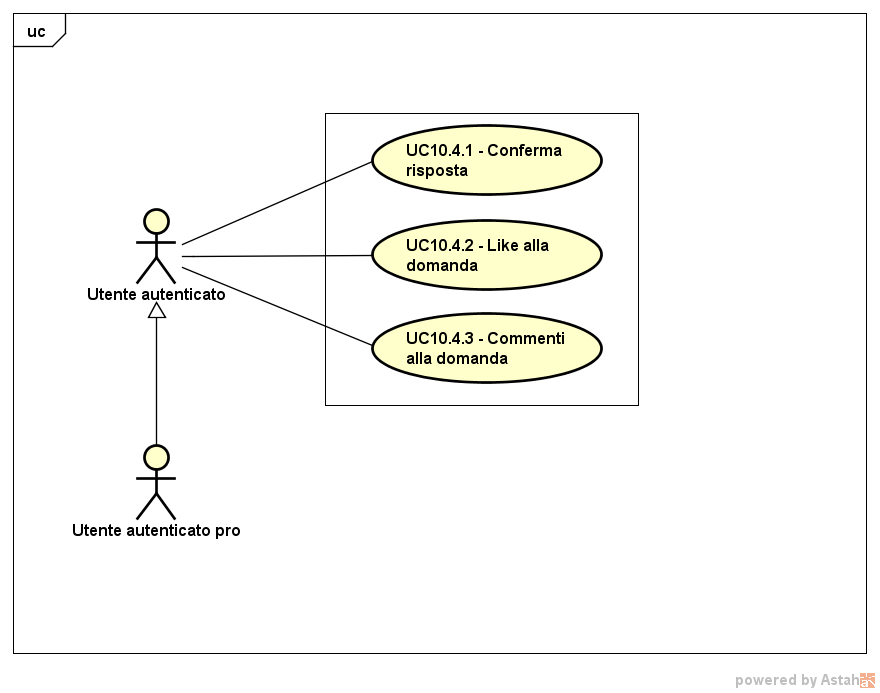
\includegraphics[scale=0.5]{UML/UC10_4.png}
	\caption{UC10.4: Inizia allenamento}
\end{figure}
\FloatBarrier
	\begin{itemize}
		\item \textbf{Attori}: utente non autenticato, utente autenticato, utente autenticato pro;
		\item \textbf{Descrizione}: l'attore può iniziare l'allenamento;
		\item \textbf{Precondizione}: l'attore ha scelto i parametri che consentiranno la creazione dell'allenamento personalizzato;
		\item \textbf{Postcondizione}: l'attore ha iniziato l'allenamento;
		\item \textbf{Scenario principale}: 
			\begin{enumerate}
				\item L'attore può confermare la risposta (UC10.4.1);
				\item L'attore può lasciare un like ad una domanda (UC10.4.2);
				\item L'attore può lasciare dei commenti alla domanda (UC10.4.3);
				\item L'attore può segnalare la domanda (UC10.4.4);
				\item L'attore può avanzare alla domanda successiva (UC10.4.5);
				\item L'utente può concludere l'allenamento (UC10.4.6).
			\end{enumerate}	
	\end{itemize}
	
\subsubsection{Caso d'uso UC10.4.1: Conferma risposta}
	\begin{itemize}
		\item \textbf{Attori}: utente non autenticato, utente autenticato, utente autenticato pro;
		\item \textbf{Descrizione}: l'attore può confermare la risposta data;
		\item \textbf{Precondizione}: l'attore ha risposto ad una domanda;
		\item \textbf{Postcondizione}: l'attore ha confermato la risposta e prosegue con l'allenamento;
		\item \textbf{Scenario principale}: l'attore conferma la risposta data alla domanda corrente.
	\end{itemize}
	
\subsubsection{Caso d'uso UC10.4.2: Like alla domanda}
	\begin{itemize}
		\item \textbf{Attori}: utente non autenticato, utente autenticato, utente autenticato pro;
		\item \textbf{Descrizione}: l'attore può lasciare un like a una domanda proposta;
		\item \textbf{Precondizione}: l'attore ha confermato la risposta ad una domanda;
		\item \textbf{Postcondizione}: l'attore ha lasciato un like alla domanda proposta;
		\item \textbf{Scenario principale}: l'attore lascia un like ad una domanda.
	\end{itemize}
	
\subsubsection{Caso d'uso UC10.4.3: Commenti alla domanda}
\label{UC10.4.3}
\begin{figure}
	\centering
	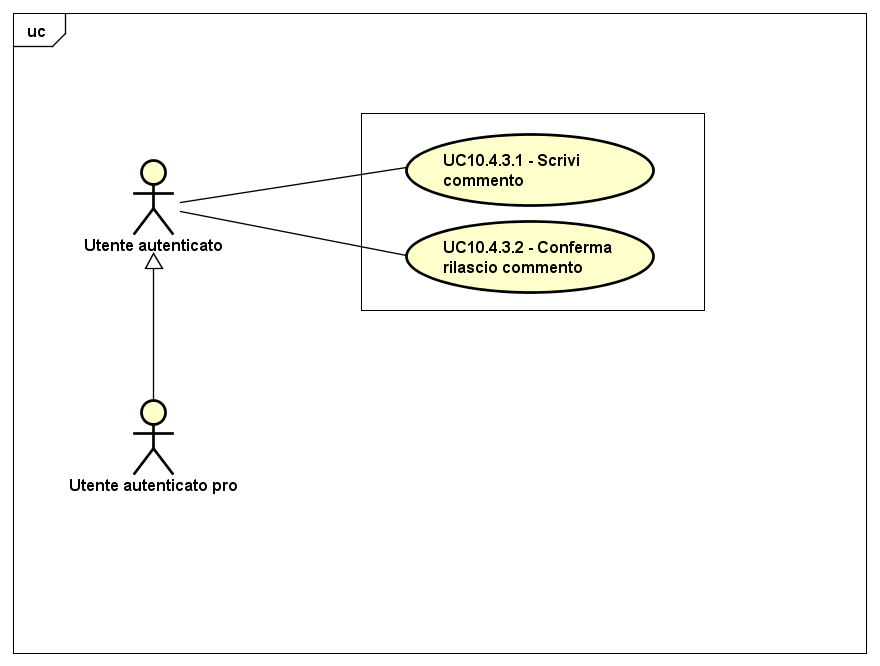
\includegraphics[scale=0.5]{UML/UC10_4_3.png}
	\caption{UC10.4.3: Commenti alla domanda}
\end{figure}
	\begin{itemize}
		\item \textbf{Attori}: utente non autenticato, utente autenticato, utente autenticato pro;
		\item \textbf{Descrizione}: l'attore può commentare una domanda;
		\item \textbf{Precondizione}: l'attore ha confermato la risposta ad una domanda;
		\item \textbf{Postcondizione}: l'attore ha commentato una domanda;
		\item \textbf{Scenario principale}:
			\begin{enumerate}
				\item L'attore scrive un commento sulla domanda (UC10.4.3.1);
				\item L'attore conferma il rilascio del commento (UC10.4.3.2).
			\end{enumerate}
	\end{itemize}
\subsubsection{Caso d'uso UC10.4.3.1: Scrivi commento}
	\begin{itemize}
		\item \textbf{Attori}: utente non autenticato, utente autenticato, utente autenticato pro;
		\item \textbf{Descrizione}: l'attore può scrivere il commento alla domanda proposta;
		\item \textbf{Precondizione}: l'attore ha confermato la risposta ad una domanda;
		\item \textbf{Postcondizione}: l'attore ha scritto un commento;
		\item \textbf{Scenario principale}: l'attore scrive un commento.
	\end{itemize}
\subsubsection{Caso d'uso UC10.4.3.2: Conferma rilascio commento}
	\begin{itemize}
		\item \textbf{Attori}: utente non autenticato, utente autenticato, utente autenticato pro;
		\item \textbf{Descrizione}: l'attore può confermare il rilascio del commento scritto;
		\item \textbf{Precondizione}: l'attore ha scritto un commento;
		\item \textbf{Postcondizione}: l'attore ha commentato una domanda;
		\item \textbf{Scenario principale}: l'attore conferma di voler inserire il commento scritto.
	\end{itemize}
\subsubsection{Caso d'uso UC10.4.4: Segnalare la domanda}
\label{UC10.4.4}
\begin{figure}
	\centering
	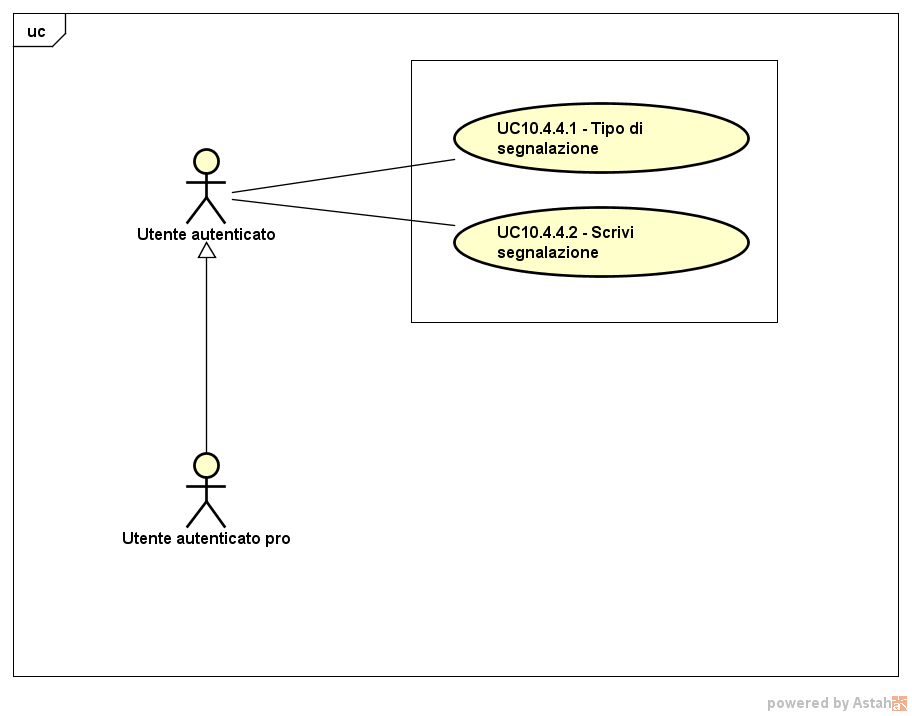
\includegraphics[scale=0.5]{UML/UC10_4_4.png}
	\caption{UC10.4.4: Segnalare una domanda}
\end{figure}
\FloatBarrier
	\begin{itemize}
		\item \textbf{Attori}: utente non autenticato, utente autenticato, utente autenticato pro;
		\item \textbf{Descrizione}: l'attore può segnalare una domanda se ritiene che sia sbagliata, mal formata oppure contenga contenuti non appropriati;
		\item \textbf{Precondizione}: l'attore ha confermato la risposta ad una domanda;
		\item \textbf{Postcondizione}: l'attore ha segnalato una domanda;
		\item \textbf{Scenario principale}:		
				\begin{enumerate}
					\item L'attore sceglie il tipo di segnalazione tra quelli proposti (UC10.4.4.1);
					\item L'attore scrive il contenuto della segnalazione (UC10.4.4.2).
				\end{enumerate}
	\end{itemize}
\subsubsection{Caso d'uso UC10.4.4.1: Tipo di segnalazione}
	\begin{itemize}
		\item \textbf{Attori}: utente non autenticato, utente autenticato, utente autenticato pro;
		\item \textbf{Descrizione}: l'attore può decidere il tipo di segnalazione tra quelli proposti;
		\item \textbf{Precondizione}: l'attore ha scelto di segnalare una domanda;
		\item \textbf{Postcondizione}: l'attore ha scelto un tipo di segnalazione;
		\item \textbf{Scenario principale}: l'attore sceglie un tipo di segnalazione.
	\end{itemize}
\subsubsection{Caso d'uso UC10.4.4.2: Scrivi segnalazione}
	\begin{itemize}
		\item \textbf{Attori}: utente non autenticato, utente autenticato, utente autenticato pro;
		\item \textbf{Descrizione}: l'attore può scrivere un commento sulla segnalazione per approfondire la motivazione;
		\item \textbf{Precondizione}: l'attore ha scelto di segnalare una domanda;
		\item \textbf{Postcondizione}: l'attore ha segnalato una domanda;
		\item \textbf{Scenario principale}: l'attore specifica perché vuole segnalare la domanda.
	\end{itemize}
\subsubsection{Caso d'uso UC10.4.5: Avanzamento domanda successiva}
	\begin{itemize}
		\item \textbf{Attori}: utente non autenticato, utente autenticato, utente autenticato pro;
		\item \textbf{Descrizione}: l'attore può avanzare alla domanda successiva dopo aver risposto alla domanda proposta; 
		\item \textbf{Precondizione}: l'attore ha risposto alla domanda proposta;
		\item \textbf{Postcondizione}: l'attore visualizza la domanda successiva;
		\item \textbf{Scenario principale}: l'attore seleziona il comando per passare alla domanda successiva.
	\end{itemize}
\subsubsection{Caso d'uso UC10.4.6: Conclusione allenamento}
	\begin{itemize}
		\item \textbf{Attori}: utente non autenticato, utente autenticato, utente autenticato pro;
		\item \textbf{Descrizione}: l'attore può concludere l'allenamento in qualunque punto dell'allenamento, anche se inizialmente aveva stabilito il numero di domande da affrontare;
		\item \textbf{Precondizione}: l'attore sta eseguendo un allenamento;
		\item \textbf{Postcondizione}: l'attore ha concluso l'allenamento e visualizza il risultato finale e le statistiche;
		\item \textbf{Scenario principale}: l'attore seleziona il comando per concludere l'allenamento.
	\end{itemize}